\documentclass[conference,letterpaper]{IEEEtran}
\IEEEoverridecommandlockouts
\usepackage{cite}
\usepackage{amsmath,amssymb,amsfonts}
\usepackage{graphicx}
\usepackage{booktabs}
\usepackage{array}
\usepackage{url}
\usepackage{xcolor}
\usepackage{tikz}
\usetikzlibrary{positioning,arrows.meta,calc}
\newcommand{\sysname}{contextctl}
\usepackage[pdfauthor={Ayan Putatunda, Suhas Jangoan},pdftitle={contextctl: Auditable, Open-Format Context Infrastructure for AI Agents},pdfcreator={},pdfproducer={},pdfsubject={},pdfkeywords={},hidelinks]{hyperref}
\begin{document}

\title{contextctl: Auditable, Open-Format\\Context Infrastructure for AI Agents}
\author{\IEEEauthorblockN{Ayan Putatunda and Suhas Jangoan}
\IEEEauthorblockA{IEEE, USA \quad \{ayan.putatunda, suhas.jangoan\}@ieee.org}}
\maketitle

\begin{abstract}
AI agents act on remembered facts, yet common memory services keep those facts in vendor schemas, keep no content-hash link to the source, and accept agent writes without review. We demonstrate \sysname{}, which manages agent context as governed data: markdown concept files in the Open Knowledge Format (OKF), Git as write gate and transaction-time record, a content-addressed evidence folder, and a rebuildable SQLite sidecar holding slowly changing dimension (SCD) Type~2 history. The demo runs the storage, versioning, indexing, and a minimal review gate with no language model, including a replay of a public dbt project's history. Accuracy, gate efficacy on model-written drafts, and the two proposed integrity properties are not evaluated here; they remain planned.
\end{abstract}

\begin{IEEEkeywords}
agent memory, data provenance, bitemporal data, version control, governance
\end{IEEEkeywords}

\section{Introduction}
During a migration, an incident-response agent learns that a critical pipeline belongs to an engineer who has left, and routes alerts to nobody for three weeks. Operators cannot say when it learned this, from what source, what it believed before, or how to restore the correct state with proof, although the right owner was in a Slack thread all along.

\textbf{The gap.} Memory services such as Mem0, Letta, and Zep~\cite{mem0,memgpt,zep} use vendor schemas, lack content-hash links to sources, and trust agent writes. Plain files are a sound base: on LoCoMo, Letta reports 74.0\% for an agent over files, above the 68.5\% Mem0 reported for its graph variant~\cite{lettafs,mem0}. The closest recent systems each cover part of the problem (Appendix~\ref{app:related}): review-gated, hash-cited knowledge (Vouch~\cite{vouch}, Assay~\cite{assay}) or bitemporal facts in SQLite (Memharness~\cite{memharness}). In their public descriptions we found none that documents all four of: (1)~custody of the source bytes behind each belief; (2)~an explicit authorization step before machine-written knowledge becomes trusted; (3)~reconstruction of what was believed, and when; (4)~serving only the context a task needs. \sysname{} targets that combination. No single mechanism is new.

\textbf{Why this is a Big Data problem.} Our measured volume is modest (256\,MB at $10^5$ synthetic concepts); the argument is operational. Evidence grows without bound, so ingestion must be incremental (watermarks) and idempotent (content addressing stores identical bytes once). Histories grow with every merge, so indexes must be derived and rebuildable rather than a second write path. Heterogeneous sources (repositories, chat, wikis) must each reduce to one evidence object. Review throughput becomes the bottleneck, so reconciliation must remove duplicates before a human sees them: in our replay, 322 of 373 drafts were classified Duplicate.

\textbf{Contributions.} (i)~A four-layer design with a precisely scoped evidence object and reconciliation rule (Sec.~\ref{sec:arch}); (ii)~a working no-model prototype and replay harness for the storage, versioning, indexing, and gate core (Sec.~\ref{sec:eval}); (iii)~replay findings that changed the specification. We label each claim \emph{measured}, \emph{demonstrated}, \emph{specified}, or \emph{planned}.

\section{Design}\label{sec:arch}
Concepts are markdown files in OKF~\cite{okf}; our OKF-MEM header profile (OKF plus memory fields) adds \texttt{actor}, \texttt{evidence}, \texttt{source}, \texttt{confidence}, \texttt{supersedes}, and validity dates. Fig.~\ref{fig:layers} shows four layers, each with one job. Generation is untrusted; curation is the only path into trusted state; the SQLite sidecar is a derived cache; serving may only propose writes, which re-enter staging.

\begin{figure}[t]
\centering
\resizebox{0.86\columnwidth}{!}{%
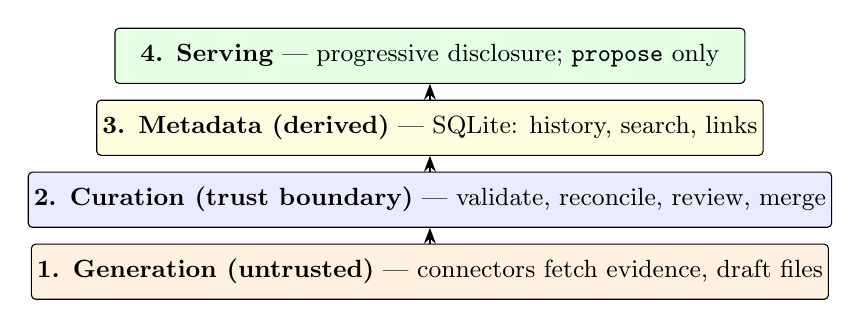
\begin{tikzpicture}[font=\small,
  layer/.style={draw, rounded corners=1.5pt, minimum width=80mm, minimum height=7mm, align=center, inner sep=2pt},
  arr/.style={-{Stealth[length=2mm]}, thick}]
\node[layer, fill=green!10] (serve) {\textbf{4. Serving} --- progressive disclosure; \texttt{propose} only};
\node[layer, fill=yellow!12, below=2mm of serve] (meta) {\textbf{3. Metadata (derived)} --- SQLite: history, search, links};
\node[layer, fill=blue!8, below=2mm of meta] (curate) {\textbf{2. Curation (trust boundary)} --- validate, reconcile, review, merge};
\node[layer, fill=orange!12, below=2mm of curate] (gen) {\textbf{1. Generation (untrusted)} --- connectors fetch evidence, draft files};
\draw[arr] (gen) -- (curate); \draw[arr] (curate) -- (meta); \draw[arr] (meta) -- (serve);
\end{tikzpicture}}
\caption{The four layers. Trusted state is layer~2: OKF files, Git history, and the evidence folder. Layer~3 can be deleted and rebuilt.}
\label{fig:layers}
\end{figure}

\textbf{Evidence object and digest scope.} At fetch time a connector stores the retained raw bytes at \texttt{evidence/}$h$, where $h$ is the SHA-256 digest of \emph{those bytes only}. The source's uniform resource identifier (URI) and retrieval time sit outside $h$, in the concept's \texttt{sources} header and in a metadata record written beside the blob when it is first stored; both are bound to the bytes only through Git history, which is why a coordinated rewrite of a header and its blob passes the digest check (P1 below). Content addressing makes a retried fetch idempotent (same bytes, same $h$, one object) and turns an edited source into a new object while the old one is kept. Behavior when a source is deleted is not yet specified.
Binary documents pass a deterministic converter whose version is recorded, so \emph{conversion} is reproducible; language-model \emph{drafting} is not, and its output is reviewed, not replayed.

\textbf{Reconciliation.} A draft $d$ is compared with the top-$k$ full-text matches ($k{=}10$) and the same-path concept $c_0$, using TF--IDF (term frequency--inverse document frequency) cosine similarity $\mathit{sim}$ and $\mathit{fields}(d,c)$, the \emph{fact} header fields that both assert with different values (in the replay, 14 dbt metric fields such as \texttt{expr} and \texttt{dimensions}). Provenance fields (\texttt{evidence}, \texttt{source}, \texttt{actor}, \texttt{confidence}, validity dates) are excluded, so a provenance-only update never raises a Conflict; with an unchanged body it is classed Duplicate and dropped, which loses the newer citation, a gap we flag. Facts stated only in the body affect only $\mathit{sim}$. The first matching rule of Table~\ref{tab:reconcile} applies. A Duplicate or Revision whose best match is a \emph{different} concept (a rename or a sibling) is held for review rather than applied.

\begin{table}[t]
\caption{Reconciliation rules, applied in order ($\theta_{\mathrm{dup}}{=}0.9$, $\theta_{\mathrm{rev}}{=}0.5$)}
\label{tab:reconcile}
\centering\scriptsize
\begin{tabular}{@{}lp{3.1cm}p{3.0cm}@{}}
\toprule
\textbf{Rule} & \textbf{Condition} & \textbf{Action}\\
\midrule
Conflict & $\mathit{fields}(d,c_0)\neq\emptyset$ & show both values; human resolves; record \texttt{supersedes}\\
Duplicate & $\max\mathit{sim}\ge\theta_{\mathrm{dup}}$, no new facts & drop draft; log match\\
Revision & $\theta_{\mathrm{rev}}\le\max\mathit{sim}<\theta_{\mathrm{dup}}$ & rewrite as edit of best match\\
New & $\max\mathit{sim}<\theta_{\mathrm{rev}}$ & add as new concept\\
\bottomrule
\end{tabular}
\end{table}

\textbf{Metadata and time.} A post-merge hook maintains one SQLite file: a slowly changing dimension Type~2 (SCD2)~\cite{kimball} table \texttt{belief\_history}, a full-text search (FTS5) index, and a table of links between concepts. \texttt{belief\_history} tracks header fields plus a digest of the body, so a body change is detected but not itemized; an owner named only in the body is not a queryable field. Valid time comes from headers, transaction time from Git. Appendix~\ref{app:bitemporal} gives measured rows, a query, and a retroactive correction. The standing test is to delete the sidecar, rebuild it, and compare a canonical row dump.

\textbf{Serving.} A specified progressive-disclosure protocol (orient, search, read, history, provenance) plus a staging-only \texttt{propose} tool, through a command-line interface (CLI), a Model Context Protocol (MCP) server~\cite{mcp}, and a plugin. Only part of the CLI is built.

\textbf{Proposed properties (hypotheses).} Under (A1)~SHA-256 collision resistance, (A2)~branch protection enforced as configured, and (A3)~byte-reproducible conversion: \emph{P1 (evidence-chain integrity)}: each hop concept$\rightarrow$commit$\rightarrow$evidence$\rightarrow$source has a check. For a coordinated header-and-blob rewrite, detection rests on Git history (see digest scope above). \emph{P2 (completeness)}: every machine-written trusted concept has a resolving chain, because the gate rejects unverifiable digests and A2 excludes other paths. On common Git hosts administrators can bypass protection, so P2 holds only where protection binds them. Signed commits would narrow the gap but are optional in the current design. A draft that sets its own \texttt{actor} or \texttt{confidence} could claim human authorship or lighter review; the gate should set \texttt{actor} from an authenticated identity (not implemented).

\section{What the Demo Shows}\label{sec:eval}
\textbf{Built:} bundle, evidence store and digest verification, a minimal reconciler and gate, the SQLite sidecar, and a rule-based notes connector. \textbf{Specified only:} repository, document, Confluence, Slack, and email connectors; the full CLI; the MCP server; the plugin. All numbers below are \emph{measured} on that built core (details and environments in Appendix~\ref{app:measure}). They show the substrate works; they are not evidence for P1, P2, accuracy, or token savings.
\begin{itemize}
\item \emph{Cost:} snapshot commits of 155\,ms at $10^4$ concepts and 634\,ms at $10^5$; full sidecar rebuilds under 1\,s; sub-millisecond point-in-time queries (synthetic data).
\item \emph{Checks:} a nine-check no-model lifecycle passed; in the replay, as-of reads matched \texttt{git show} in 665/665 cases and the rebuilt sidecar matched the incremental one row for row.
\item \emph{Replay of the public dbt Jaffle Shop history} (scripted admission, no model): 373 drafts gave 16 New, 322 Duplicate, 24 Revision, and 11 Conflict; each Conflict corresponds to an upstream edit of \texttt{dimensions} or \texttt{expr}.
\end{itemize}

\textbf{What the replay taught us.} (a)~Checking Conflict against every candidate flagged 359 of 373 drafts, so it is now scoped to the same path. (b)~A coordinated header-and-blob rewrite passed the digest check and showed only as an uncommitted Git change. (c)~The full governed bundle cost about $4.6\times$ the tokens of the raw sources, because digests and URIs tokenize poorly. (d)~Reverting one merge conflicted with a later merge of the same files.

\section{Limitations and Planned Evaluation}\label{sec:disc}
This demo has no accuracy result. Planned (not preregistered) research questions (RQs): \textbf{RQ1} accuracy parity, not gains, with memory services on LoCoMo and LongMemEval~\cite{locomo,longmemeval}; \textbf{RQ3} whether disclosure tiers beat flat retrieval in tokens at equal correctness, given (c); \textbf{RQ5} gate efficacy on model-written and adversarial drafts; \textbf{RQ6} systematic tamper detection. The scale check uses two sizes of single-template synthetic data and is not a scaling result. The replay has no model and no human reviewer, and the opening Slack/Confluence scenario is not tested. Retaining evidence conflicts with deletion rights, and harvesting Slack or email keeps employees' messages, which raises consent and access questions.

\textbf{Conclusion.} \sysname{} is a partially built stack for managing agent context as governed data. The demo shows its storage, versioning, indexing, and gate core working on open components, and a model-free replay finding specification bugs.

\section*{AI Usage Disclosure}
Large language model (LLM) tools assisted with (1)~writing and debugging the prototype and benchmark harnesses, (2)~drafting and revising the manuscript, including simulated peer review, and (3)~finding and checking related work. The authors verified all AI-assisted output and take full responsibility for the content and references. All reported measurements come from scripts that were executed, not from model output.

\appendices
\section{Closest Systems}\label{app:related}
Memory services and Git-versioned reasoning tools (GCC, GitOfThoughts~\cite{gcc,got}) address adjacent problems. Closer systems realize pieces of our design: Vouch is a Git-native, review-gated knowledge base whose claims cite sources, exposed through MCP and a CLI~\cite{vouch}; Memharness keeps bitemporal facts with provenance in SQLite behind MCP~\cite{memharness}; a preprint describes a replayable bitemporal memory substrate~\cite{bpma}; Git-bound memory for coding agents uses merge as the admission gate~\cite{rekal}; Assay binds claims to content-hashed evidence reviewed before merge~\cite{assay}. Table~\ref{tab:compare} uses only those descriptions (``--'': none documented, not a verified absence); we ran no systematic survey.

\begin{table}[h]
\caption{Closest systems (public descriptions, accessed Oct.\ 2026). The \sysname{} column is design intent; see Sec.~\ref{sec:eval} for what is built.}
\label{tab:compare}
\centering\scriptsize
\setlength{\tabcolsep}{2.5pt}
\begin{tabular}{@{}lcccc@{}}
\toprule
\textbf{Property} & \textbf{Vouch} & \textbf{Memharness} & \textbf{Assay} & \textbf{\sysname{}}\\
\midrule
Review gate before belief & yes & -- & yes & built (min.)\\
Content-hash evidence binding & yes & --$^{a}$ & yes & built\\
Bitemporal / SCD2 sidecar & -- & yes & -- & built (min.)\\
Governed Slack/wiki ingestion & -- & -- & -- & specified\\
Specified reconciliation rules & -- & -- & -- & built (min.)\\
Token-tiered serving & -- & -- & -- & specified\\
\bottomrule
\end{tabular}\\[2pt]
{\raggedright\scriptsize $^{a}$Per-fact provenance; we do not equate it with content-hash binding.\par}
\end{table}

\section{Worked Bitemporal Example (Measured Rows)}\label{app:bitemporal}
Upstream Jaffle Shop commit \texttt{a75613b} (2024-07-04) changed the \texttt{food\_revenue} expression from \texttt{= 1} to \texttt{is true}; it reached the mainline in a 2024-09-12 merge, and a 2025-07-01 merge changed it again. The replay held that harvest as a Conflict on \texttt{expr} until scripted approval. Resulting rows (abbreviated):

\begin{center}\scriptsize
\begin{tabular}{@{}llllll@{}}
\toprule
old & new & valid\_from & valid\_to & snapshot\\
\midrule
-- & \texttt{= 1} & 2023-08-30 & 2024-09-12 & 16c4a6f\\
\texttt{= 1} & \texttt{is true} & 2024-09-12 & 2025-07-01 & 6104f5c\\
\texttt{is true} & bare boolean & 2025-07-01 & open & 11917f9\\
\bottomrule
\end{tabular}
\end{center}

\noindent ``What was the expression on $t$?'' (valid time) is one range query:
\texttt{SELECT new\_value FROM belief\_history WHERE concept=:c AND field='expr' AND valid\_from<=:t AND (valid\_to IS NULL OR valid\_to>:t)}; for $t$ = 2024-06-01 it returns \texttt{= 1} and for 2025-01-01 \texttt{is true}, matching the replay. The transaction-time question (what the bundle said at a snapshot) is an as-of read at that commit.

\textbf{Retroactive correction (derived from the hook's rule, not run).} The fix actually applied from 2024-07-04, not 2024-09-12. If the admitted draft carries \texttt{valid\_from: 2024-07-04}, the hook closes row~1 at 2024-07-04 and opens row~2 at 2024-07-04 while its snapshot (transaction time) stays 2024-09-12. A valid-time query for 2024-08-01 then returns \texttt{is true}, but an as-of read of the bundle on 2024-08-01 still returns \texttt{= 1}: the two time axes differ exactly over the period in which the agent was wrong. A later commit that edits \emph{only} \texttt{valid\_from} is recorded in Git but not in \texttt{belief\_history} in the current harness, a gap we flag.

\textbf{Rollback.} Reverting only the 2024-09-12 merge failed, since the 2025-07-01 merge edited the same files; reverting it and the two later merges restored it.

\section{Measurement Details}\label{app:measure}
\textbf{Microbenchmarks} (single vCPU; Git~2.43, SQLite~3.45, Python~3.12; medians): bundles of $10^2$--$10^4$ concepts, 30 commits touching 1\% of files; at $10^4$, snapshot commit 155.1\,ms, as-of read and revert about 3--5\,ms, sidecar rebuild 0.47\,s.
\textbf{Two-size scale check} (same class of environment; $10^4$ and $10^5$ single-template concepts; 10 commits touching 0.1\%): at $10^5$, history rebuild 0.67\,s, FTS5 build 4.3\,s, link extraction 1.7\,s, snapshot commit 634\,ms; storage 88/25/143\,MB (bundle/Git/sidecar). Path-scoped staging was not measured.
\textbf{Replay} (8 vCPU VM; Git~2.47, SQLite~3.53; Jaffle Shop pinned at commit \texttt{7be2c58}; 7 repeats, identical counts): 25 steps, 7 merges, 22 final concepts. Tokens (tiktoken \texttt{cl100k\_base}, medians): orient+search+read 2{,}026; full bundle 30{,}460; raw dbt files 6{,}579; a full concept read 1{,}339 versus 190 for its body; a body-only orient+search+read variant 880. No flat-retrieval baseline was run.

\begin{thebibliography}{00}\footnotesize
\bibitem{okf} S. McVeety and A. Hormati, ``How the Open Knowledge Format can improve data sharing,'' Google Cloud Blog, Jun.\ 12, 2026.
\bibitem{kimball} R. Kimball and M. Ross, \emph{The Data Warehouse Toolkit}, 3rd ed. Wiley, 2013.
\bibitem{mem0} P. Chhikara, D. Khant, S. Aryan, T. Singh, and D. Yadav, ``Mem0: Building production-ready AI agents with scalable long-term memory,'' in \emph{Proc.\ ECAI}, FAIA vol.~413, 2025, pp.~2993--3000.
\bibitem{lettafs} Letta, ``Benchmarking AI agent memory: Is a filesystem all you need? Letta blog, Aug.\ 12, 2025. [Online]. Available: letta.com/blog/benchmarking-ai-agent-memory
\bibitem{memgpt} C. Packer \emph{et al.}, ``MemGPT: Towards LLMs as operating systems,'' arXiv:2310.08560, 2023.
\bibitem{zep} P. Rasmussen \emph{et al.}, ``Zep: A temporal knowledge graph architecture for agent memory,'' arXiv:2501.13956, 2025.
\bibitem{vouch} ``vouch: A git-native, review-gated knowledge base for AI agents,'' GitHub repository vouchdev/vouch, accessed Oct.\ 2026.
\bibitem{assay} O. S. Tiwari \emph{et al.}, ``Assay: Claims that decay with the code. Content-addressed evidence graphs for accountable AI-assisted software delivery,'' arXiv:2609.36170, 2026.
\bibitem{memharness} ``memharness: A bi-temporal, provenance-carrying memory primitive for AI agents,'' GitHub repository las7/memharness, accessed Oct.\ 2026.
\bibitem{mcp} Anthropic, ``Introducing the Model Context Protocol,'' Nov.\ 2024. [Online]. Available: anthropic.com/news/model-context-protocol
\bibitem{locomo} A. Maharana \emph{et al.}, ``Evaluating very long-term conversational memory of LLM agents,'' in \emph{Proc.\ ACL}, 2024, pp.~13851--13870.
\bibitem{longmemeval} D. Wu \emph{et al.}, ``LongMemEval: Benchmarking chat assistants on long-term interactive memory,'' in \emph{Proc.\ ICLR}, 2025.
\bibitem{gcc} J. Wu \emph{et al.}, ``Git Context Controller: Manage the context of LLM-based agents like Git,'' arXiv:2508.00031, 2025.
\bibitem{got} P. C. Shekar \emph{et al.}, ``GitOfThoughts: Version-controlled reasoning and agent memory you can replay, diff, and merge,'' arXiv:2606.14470, 2026.
\bibitem{bpma} M. Vidrih, ``Who knew what, when, and why: A replayable, bitemporal memory substrate for AI agents,'' preprint, 2026, doi:10.5281/zenodo.21654958.
\bibitem{rekal} F. Guo, ``Why Git is the memory solution for the agentic development lifecycle,'' arXiv:2607.14390, 2026.
\end{thebibliography}
\end{document}
